\chapter{Background knowledge}

\label{ch:Background knowledge}

\setlength{\parindent}{4em}
\setlength{\parskip}{1em}
\renewcommand{\baselinestretch}{1.5}

\section{Background knowledge}

\subsection {Electroencephalography (EEG)}

\hspace{1.5cm} EEG is a technique for studying the electrical activities within the brain using electrodes that attached to the surface of the scalp. Wires attach these electrodes to a machine, which records the electrical impulses. The results are either printed out or displayed on a computer screen. A different pattern of electrical impulses can denote the various form of epilepsy\cite{ref9}. It is also used to diagnose sleep disorders, coma, encephalopathies, and brain death.\par
Derivatives of the EEG technique include evoked potentials (EP), which involves averaging the EEG activity time-locked to the presentation of a stimulus of some sort (visual, somatosensory, or auditory). Event-related potentials (ERPs) refers to averaged EEG responses that are time-locked to more complex processing of stimuli. While Steady state visually evoked potential (SSVEP) refers to stable EEG waveform which has the same or multiple of the frequency of the visual stimulus



\begin{figure}[h]
	\centering
	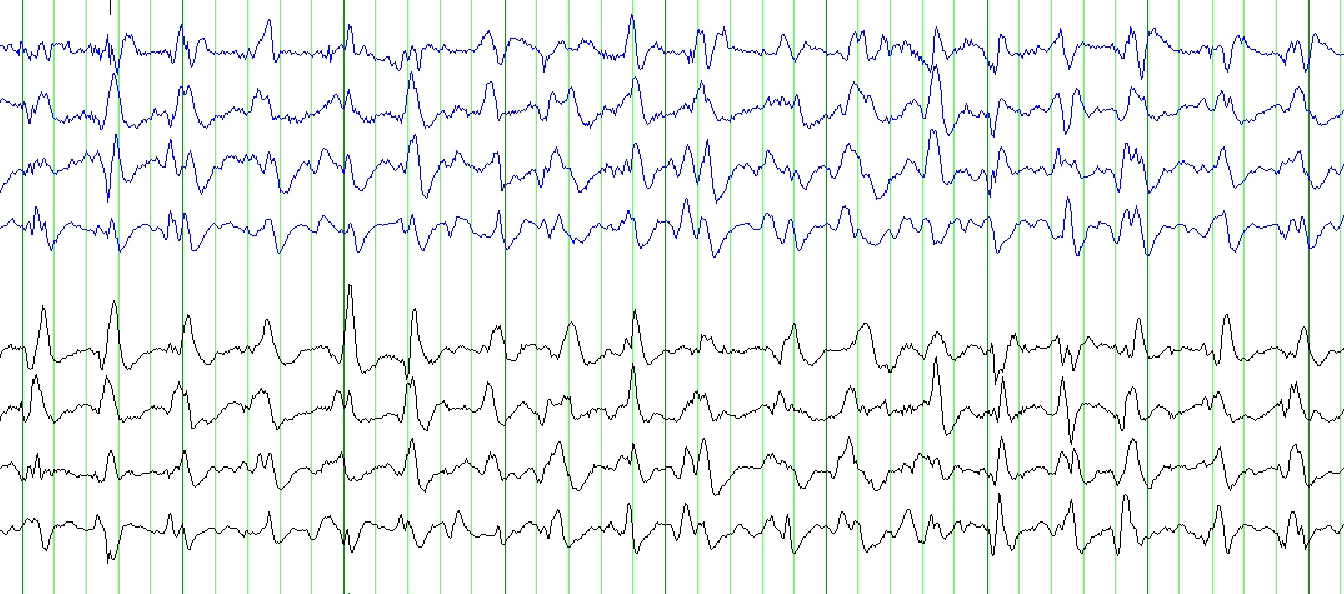
\includegraphics[scale = 0.5]{chapter3/31.pdf}
	\caption{EEG signal}
\end{figure}
\newpage

\subsection{Event-related potential (ERPs)}

\hspace{1.5cm} Event-related potentials (ERPs) are very small voltages generated in the brain structures in response to specific events or stimuli. They measure brain response that is directed result of a specific sensory, cognitive or motor event. To see the brain's response to a stimulus, the experimenter must conduct many trials (usually in the order of 100 or more) and average the results together, causing random brain activity to be averaged out and the relevant waveform to remain, these stimuli can be visual, auditory, tactile and even olfactory and gustatory.


\begin{figure}[h]
	\centering
	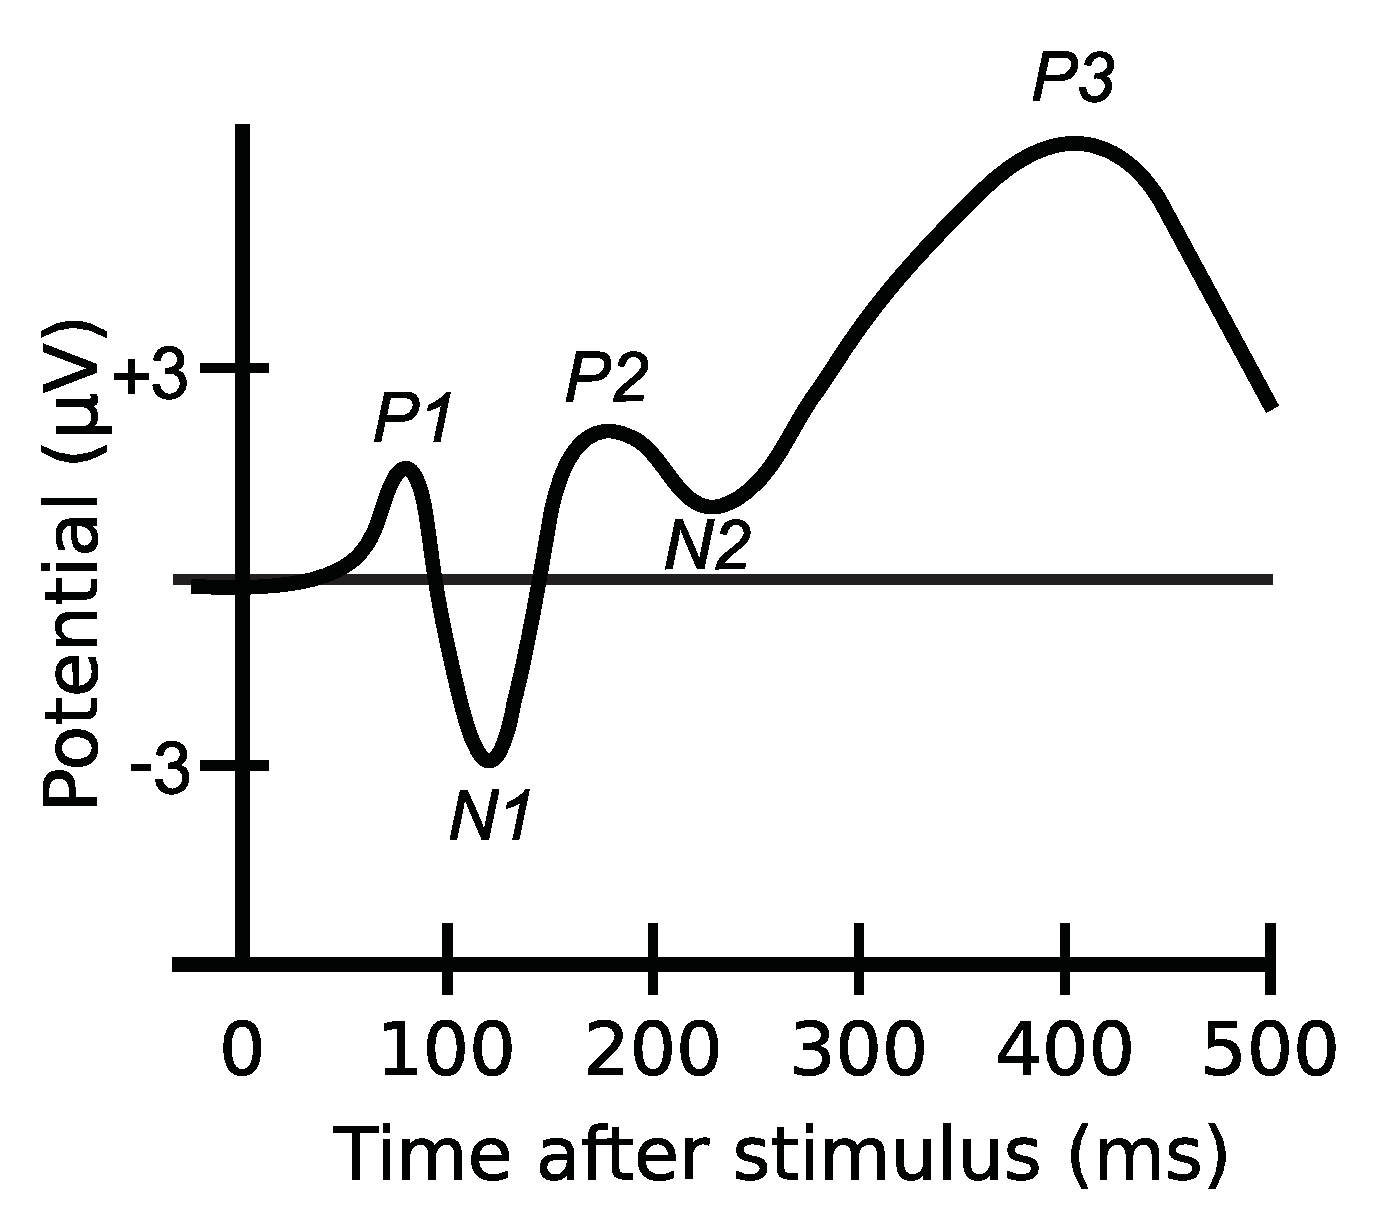
\includegraphics[scale = 0.3]{chapter3/32.pdf}
	\caption{Averaged ERP waveform}
\end{figure}

\newpage
\subsection{Steady state visually evoked potential (SSVEP)}

\hspace{1.5cm}  Steady State Visually Evoked Potentials or SSVEPs are EEG signals that are natural responses to visual stimulation. when the subject is in meditation state the brain will generate a stable EEG waveform. But when the subject's retina is stimulated by a visual stimulus which ranging from 3.5 Hz to 75 Hz, the brain generates electrical activity at the same or multiple of the frequency of the visual stimulus.\par


\subsection{Cerebral Cortex}

\hspace{1.5cm} The human brain consists of several parts. The part that makes human more intelligent than any animals are Cerebrum. The cerebrum is the largest part of human brain. The physician divides the cerebrum into four parts. There is frontal lobe, parietal lobe, temporal lobe and occipital lobe. The frontal lobe locates at the front of the brain. It controls the creative thought, thinking, problem solving and muscle movements. The parietal lobe locates behind the frontal lobe. It involved in the visual functions, languages, reading and sensory controls. Temporal lobe situates beneath both frontal lobe and parietal lobe. It implicates in control memories, speech and hearing languages. Occipital lobe locates at occipital. it related with a human vision controls. Due to our project study about the human visualization, so we focus on the occipital lobe

\begin{figure}[h]
	\centering
	\includegraphics[scale = 0.32]{chapter3/33.pdf}
	\caption{1.Frontal lobe, 2.Parietal lobe, 3.Temporal lobe, 4.Occipital lobe}
\end{figure}

\newpage
\subsection{Feature scaling (normalization)}

\hspace{1.5cm} Feature scaling is used to normalize the range of independent variables or features of data to have the properties of a standard normal distribution. to make in some machine learning algorithms work properly. it is usually performed while in the data pre-processing step. The calculation is determined the distribution mean and standard deviation for each feature. Next, we subtract the mean from each feature. Then divide the values which already subtracted by mean, by its standard deviation.\cite{ref10}

\[x' = {x-{\overline{x}} \over {\sigma}}\]

\subsection{Uniform distribution\cite{ref11}}

\hspace{1.5cm} The Uniform or Rectangular distribution has random variable  restricted to a finite interval  and has  has constant density over the interval.
\begin{figure}[h]
	\centering
	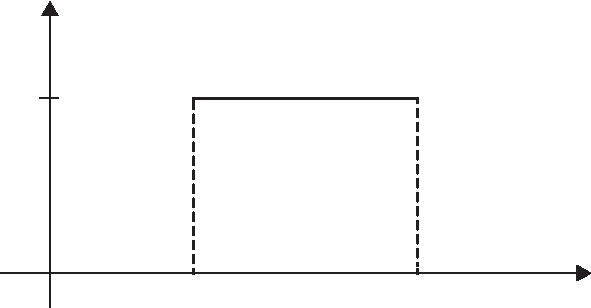
\includegraphics[scale = 0.8]{chapter3/34.pdf}
	\caption{An illustrate of uniform distribution}
\end{figure}

\newpage
The function f(x) is defined by:

\[f(n) = \left\{ 
\begin{array}{l l}
  {1 \over b-a} & \quad \mbox{if $a$ $\leq x$ $\leq b$}\\
  0 & \quad \mbox{$otherwise$}\\ \end{array} \right. \]

\subsection{10/20 international system}
\hspace{1.5cm} The 10/20 international system is a recognized method to describe and apply the location of scalp electrodes in the context of EEG test. This system is based on the relationship between the location of an electrode and the underlying area of cerebral cortex. The 10/20 international system refers to the actual distance between adjacent electrodes are either 10 \% or 20 \% of the total front-back or right-left distance of the skull. Each site has letters to identify the lobe and a number to identify the hemisphere location. The letters F stands for frontal lobe, T is temporal lobe, C is central lobe, P is parietal lobe, and the last one is O means occipital lobe. Even numbers refer to electrode positions on the right hemisphere and odd numbers refer to the electrode positions on the left hemisphere.

\begin{figure}[h]
	\centering
	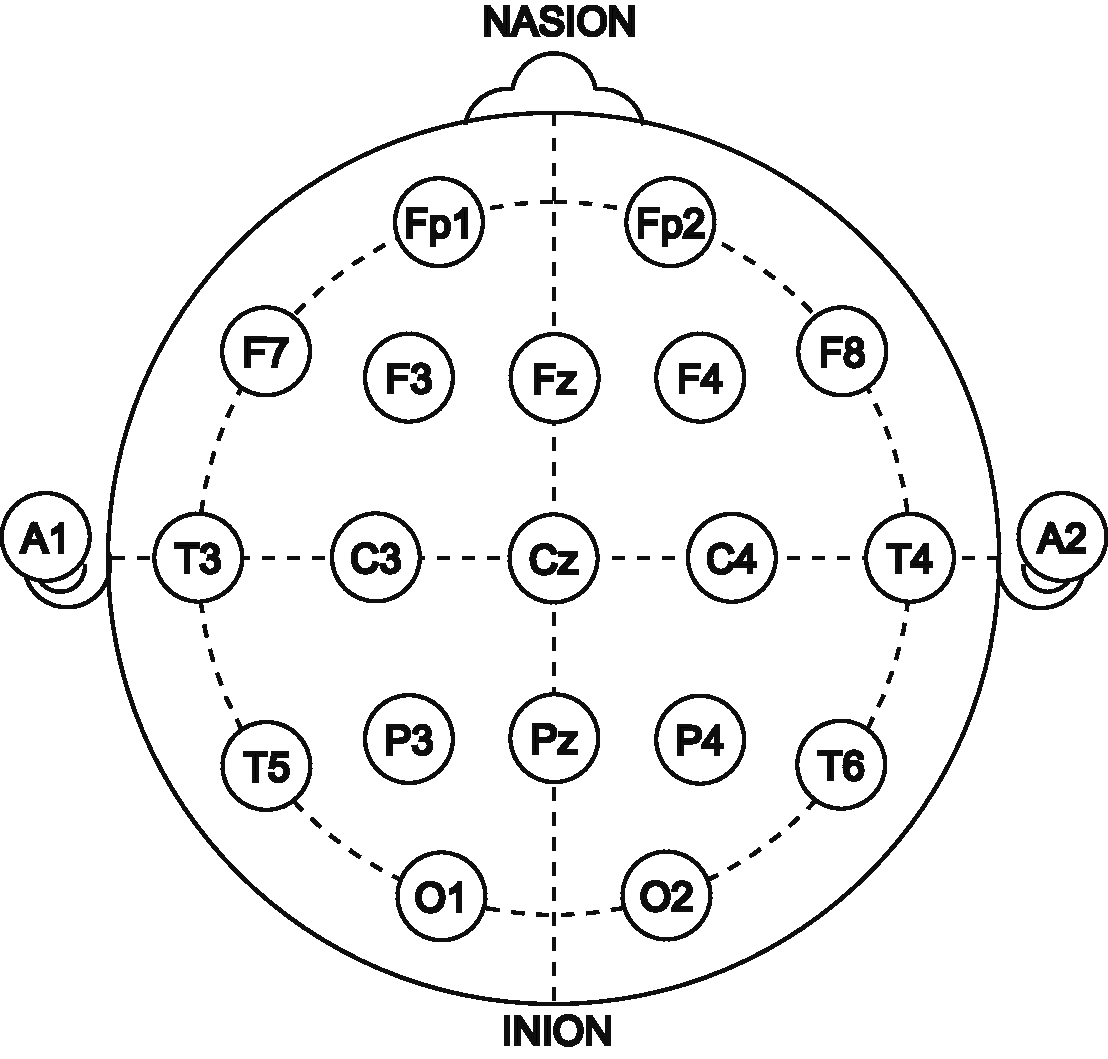
\includegraphics[scale = 0.4]{chapter3/35.pdf}
	\caption{International 10-20 locations system}
\end{figure}

\newpage
\subsection{Standard deviation}
\hspace{1.5cm} Standard deviation(SD) is measuring a distribution of the collection of data.if the SD is high, the distribution is high. if the SD is low, the distribution is low.

\subsection{Low-pass filter}
\hspace{1.5cm}The Low-pass filer only allow the frequency signal that is below  cut-off frequency
\begin{figure}[h]
	\centering
	\includegraphics[scale = 0.14]{chapter3/lowpass.pdf}
	\caption{Low-pass filter}
\end{figure}

\subsection{High-pass filter}
\hspace{1.5cm}The High-pass filter only allow the frequency signal that is higher than cut-off frequency
\begin{figure}[h]
	\centering
	\includegraphics[scale = 0.14]{chapter3/highpass.pdf}
	\caption{High-pass filter}
\end{figure}

\subsection{Band-pass filter}
\hspace{1.5cm}The Band-pass filter only allow the frequency signal that is in the specified range
\begin{figure}[h]
	\centering
	\includegraphics[scale = 0.14]{chapter3/bandpass.pdf}
	\caption{Band-pass filter}
\end{figure}

\newpage
\subsection{EEG band}
\hspace{1.5cm}EEG band determined as a fixed range of wave frequency and amplitudes over a time scale. In Scientific field classify into 5 types. that are,

1.Delta band is the lowest frequency in the range of 0-3 Hz. It occurs during deep sleep

2.Theta band is in the frequency range between 4-7 Hz. We can investigate the situation of intuitive,creative and imagery. 

3.Alpha band is in the frequency range between 8-12 Hz. It occurs during the situation that our mind calm,so we can obtain the strongest EEG brain signal in this frequency range.

4.Beta band is in the frequency range between 12-30 Hz. We can investigate this band at the situation of memory and problem-solving.

5.Gamma band is in the frequency range between 30-100 Hz. This wave may be implicated in creating the unity of conscious perception. 

\subsection{Fourier transform}
The Fourier transform is the mathematical model which uses to transform from the time signal into the frequency domain.

\subsection{Short-time Fourier transform} 
The short-time Fourier transform(STFT) divide a long time signal into shorter groups before computing the Fourier transform on each group.

\newpage
\section{Material background}

\subsection{Emotiv EPOC headset\cite{ref12}}

\hspace{1.5cm} The wireless headset Emotiv EPOC research edition, it records EEG data in 14 channel of International 10-20 Locations system with Sequential sampling rate at 128 per second (2048 Hz internal) with resolution 14 bit (16 bit Analog to digital converter, 2-bit instrumental noise floor discarded), the bandwidth is in range 0.2 to 45 Hz with digital notch filters at 50Hz and 60 Hz
\begin{figure}[h]
	\centering
	\includegraphics[scale = 0.09]{chapter3/36.pdf}
	\caption{Emotive Headset}
\end{figure}

\newpage
\subsection{Gravitech Gerora LED\cite{ref13}}

\hspace{1.5cm} The full-color Light-emitting diode (LED) driver which is use for stimulating the subject has an LED light WS2812 model mounted on. It can chain connected with the same model. It can be controlled by a programmed Arduino. The luminous intensity is 550 to 700 mega candela for red, 1100-1400 mcd for green, and 200-400 mcd for blue.
\begin{figure}[h]
	\centering
	\includegraphics[scale = 0.3]{chapter3/37.pdf}
	\caption{Gravitech Gerora LED base on WS2812}
\end{figure}
\subsection{Arduino UNO\cite{ref14}}

\hspace{1.5cm} The Arduino Uno is a microcontroller board based on the ATmega328 that is an open source platform. It has 14 input/output pins6 analog inputs, a 16 MHz quartz crystal, a USB connection, a power jack, an ICSP header and a reset button, The USB connection for upload the software into the Arduino and VCC or supply for connecting the peripheral circuit.   
\begin{figure}[h]
	\centering
	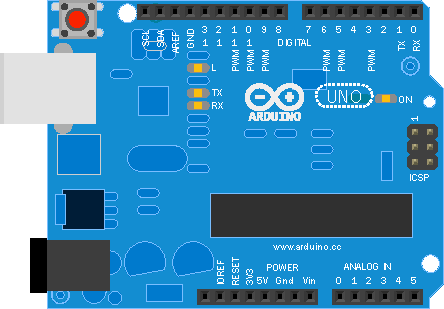
\includegraphics[scale = 0.6]{chapter3/38.pdf}
	\caption{Illustrate of Arduino UNO board}
\end{figure}



